Funkcja \prawo{251} $\Phi \colon \mathbb A \times \mathbb A \to \mathfrak K$ jest \wcht{dwuafiniczna}, jeśli ,,ustalenie jednego argumentu daje afiniczną funkcję''.
\wcht{Symetryczna}: $\Phi(\dot p, \dot q) = \Phi(\dot q, \dot p)$.
Istnieje $\dot o \in \mathbb A$, dwuliniowa $f \colon V \times V \to \mathfrak K$ oraz liniowe $l, l' \colon V \to \mathfrak K$, że khm-1.
\wcht{Funkcja kwadratowa} $Q$: postaci $Q(\dot p) = \Phi(\dot p, \dot p)$ dla khm-1 i $l = l'$.
Jeśli $q(x) = f(x,x)$, to rzędem $Q$ jest rząd $q$.
Punkt $\dot p \in \mathbb A$ jest \wcht{środkowy} dla kwadratowej $Q$, jeśli $Q (\dot p + y ) = Q(\dot p) + q(y)$; zbiór wszystkich to $C(Q)$.
Jak ich szukać?
Twierdzenie 1/216 mówi, że $C(Q)$ jest pusty tylko dla zdegenerowanej $q$ ($\rank q<n$).
\[
	\Phi(\dot o + x, \dot o + y) = f(x,y) + l(x) + l'(y) + \Phi(\dot 0, \dot o)
\]

Jeśli $Q$ jest funkcją kwadratową rzędu $r \ge 0$ na $n$-wymiarowej p. afinicznej $\mathbb A$ nad $\mathfrak K$ bez punktów środkowych (wtedy $r < n$), to istnieje układ współrzędnych, w których $Q$ zapisuje się w postaci $Q(\dot o + x) = \sum_{k=1}^r \alpha_k x_k^2 + 2x_{r+1}$, gdzie $\alpha_k \neq 0$ to skalary; jądrem $q$ są te $x \in V$, że $x_1 = \dots = x_r = 0$.
Jeśli $\dot o$ jest środkowy, to $Q$ ma podobną postać, ale $Q(\dot o) $ jest zamiast $2 x _{r+1}$.
Są jeszcze kwadratowe na euklidesowej. %251-4

Każdej \prawo{2 / 52} funkcji kwadratowej na afinicznej $\mathbb A$ odpowiada \wcht{kwadryka} $S_Q = \{\dot{p} \in \mathbb  A : Q(\dot p) = 0\}$.
Załóżmy, że $\rank S_Q = r = \rank q > 0$ oraz $n \ge 2$, a $S_Q \neq \varnothing$.
Kwadryka jest \wcht{p. podwójną}, jeśli jest afiniczną podp. $\mathbb A$.
Jeśli nie, to $S_{Q_1} = S_{Q_2} \Ra Q_2 = \lambda Q_1$ dla $\lambda \in \mathbb R \setminus \{0\}$.
Punkt $\dot o \in \mathbb A$ to \wcht{środek} $S_Q$, jeśli $\dot o + x \in S_Q$ pociąga $\dot o - x \in S_Q$.
Każda kwadryka ma postać I, I' lub II.
\wcht{Typy}: elipsoida ($I_{n,n}$), hiperboloida ($I_{s,n}$, $s < n$), paraboloida eliptyczna ($II_{n-1,n-1}$), hiperboliczna ($II_{s, n-1}$ dla $s < n-1$); walce ($I_{s,r}$ lub $I'_{s,r}$ dla $r < n$, $II_{s,r}$ dla $ r< n-1$) i stożki ($I'_{s,n}$).
Każdy typ ma swoje naturalne ograniczenia.
Typ I: $0 < s \le r$, typ I': $r/2 \le s \le r$, typ II: $r/2 \le s \le r < n$.
\[
	I_{s,r} : x_1^2 + \dots + x_s^2 - x_{s+1}^2 - \dots - x_r^2 = 1 \spk
	I'_{s,r} : \dots = 0,\, r/2 \le s \le r \spk
	II_{s,r} : x_1^2 + \dots + x_s^2 - x_{s+1}^2 - \dots - x_{r}^2 = -2 x_{r+1}
\]

\begin{center}
\fbox{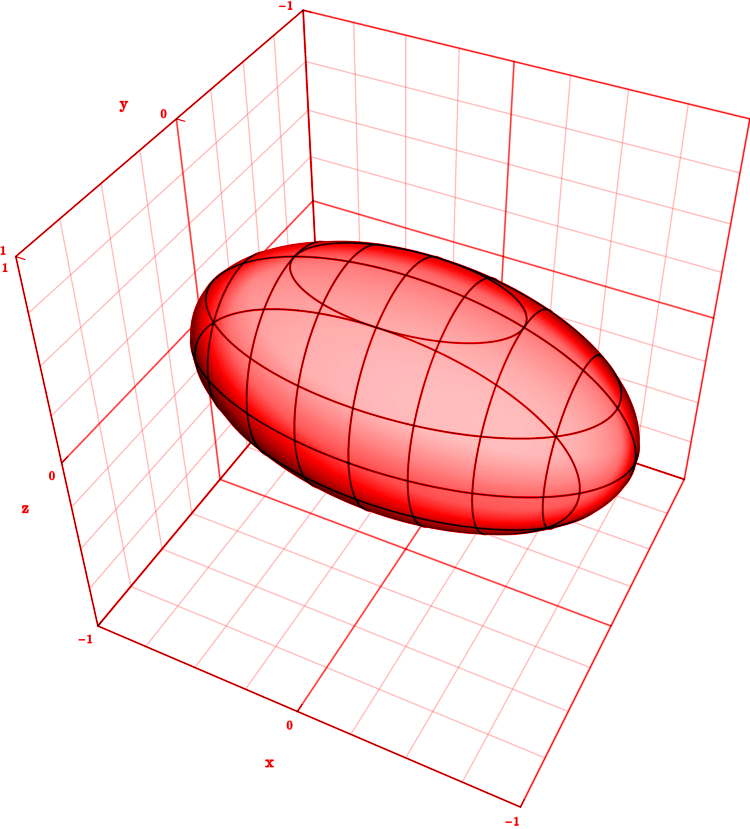
\includegraphics[height=0.090\columnwidth]{img/q1.png}}
\fbox{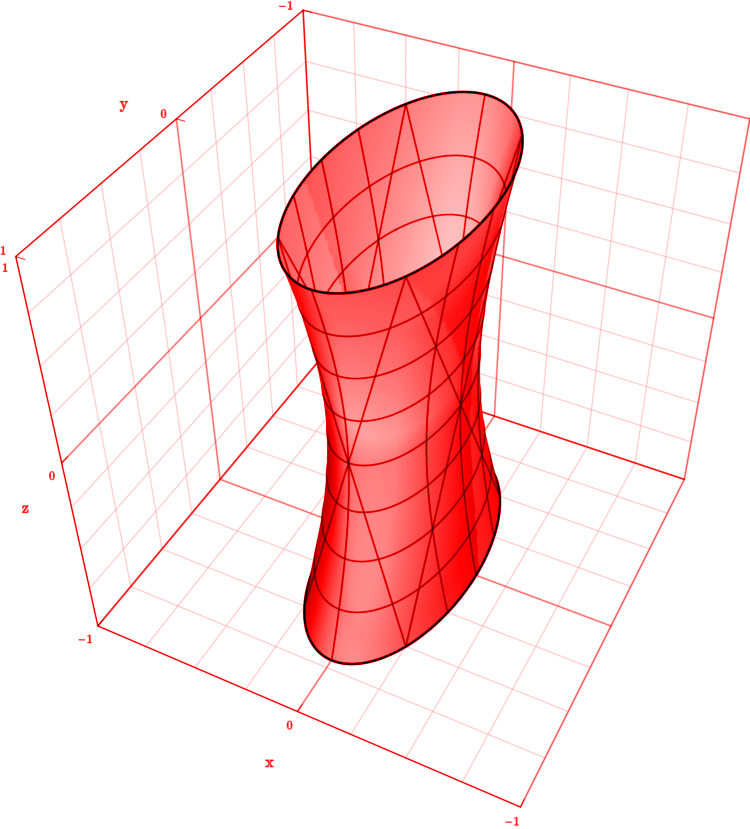
\includegraphics[height=0.090\columnwidth]{img/q2.png}}
\fbox{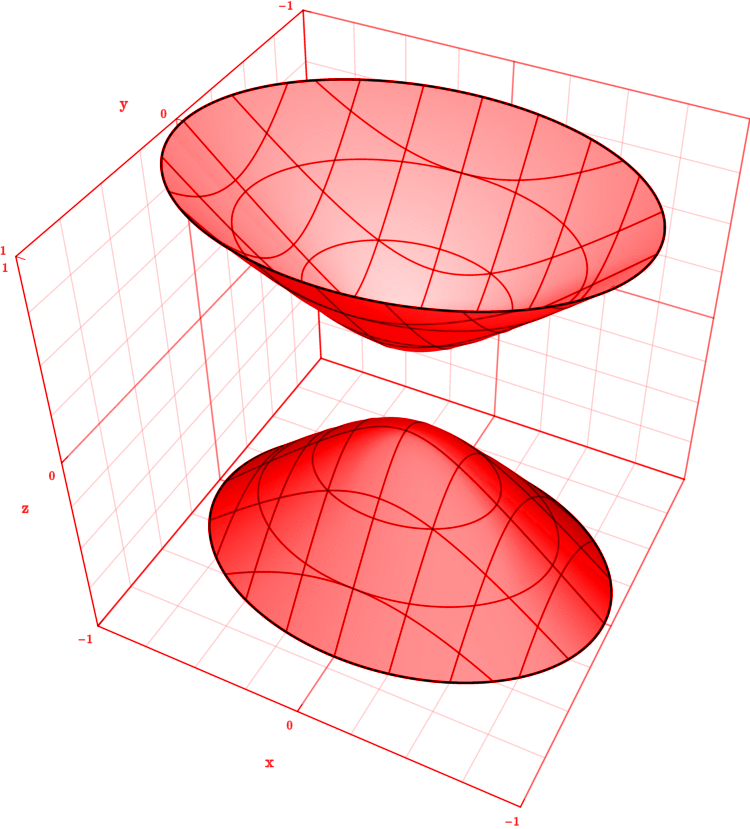
\includegraphics[height=0.090\columnwidth]{img/q3.png}}
\fbox{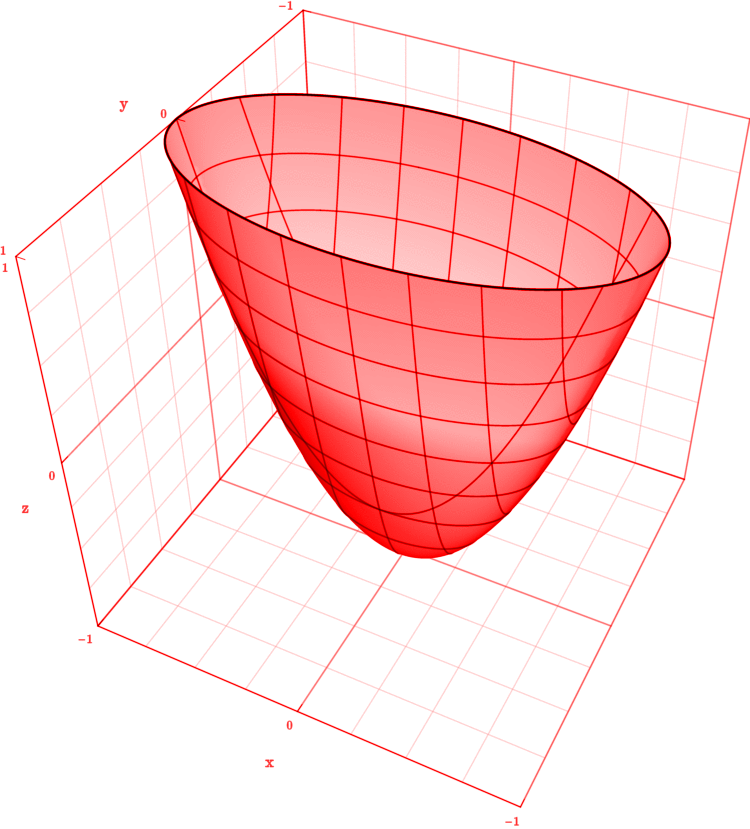
\includegraphics[height=0.090\columnwidth]{img/q4.png}}
\fbox{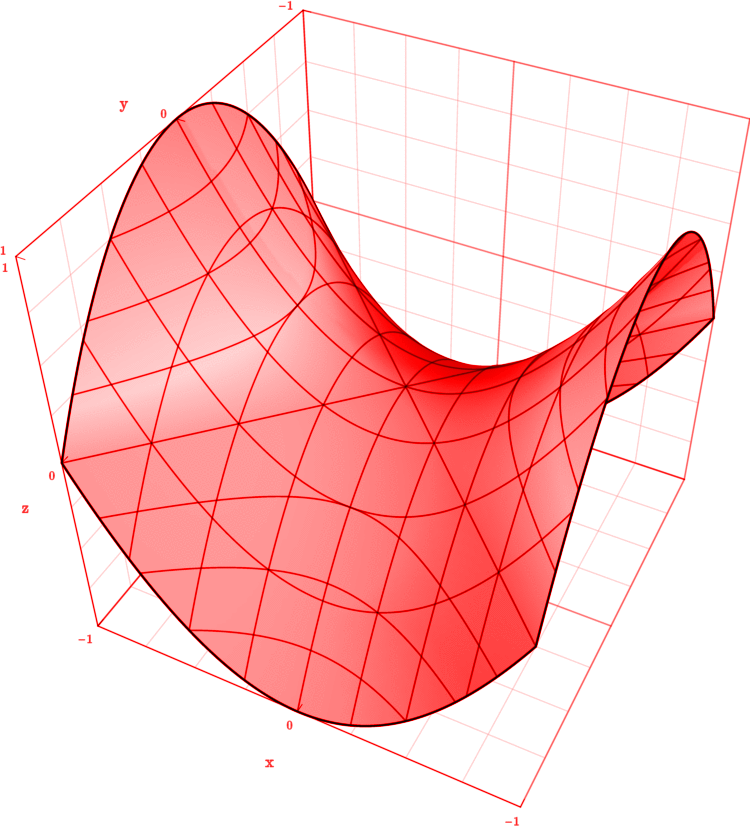
\includegraphics[height=0.090\columnwidth]{img/q5.png}}
\fbox{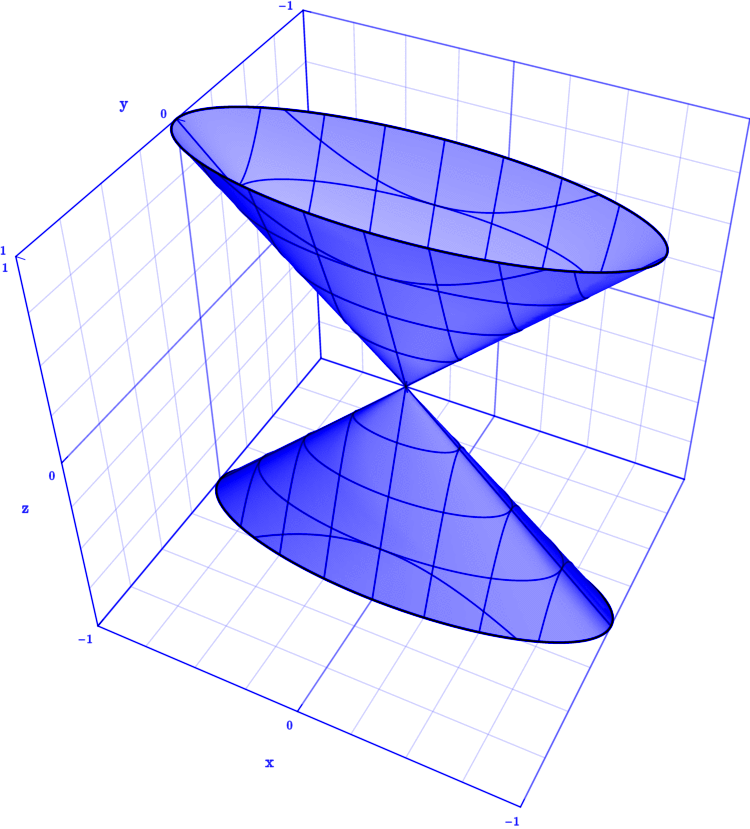
\includegraphics[height=0.090\columnwidth]{img/q6.png}}
\fbox{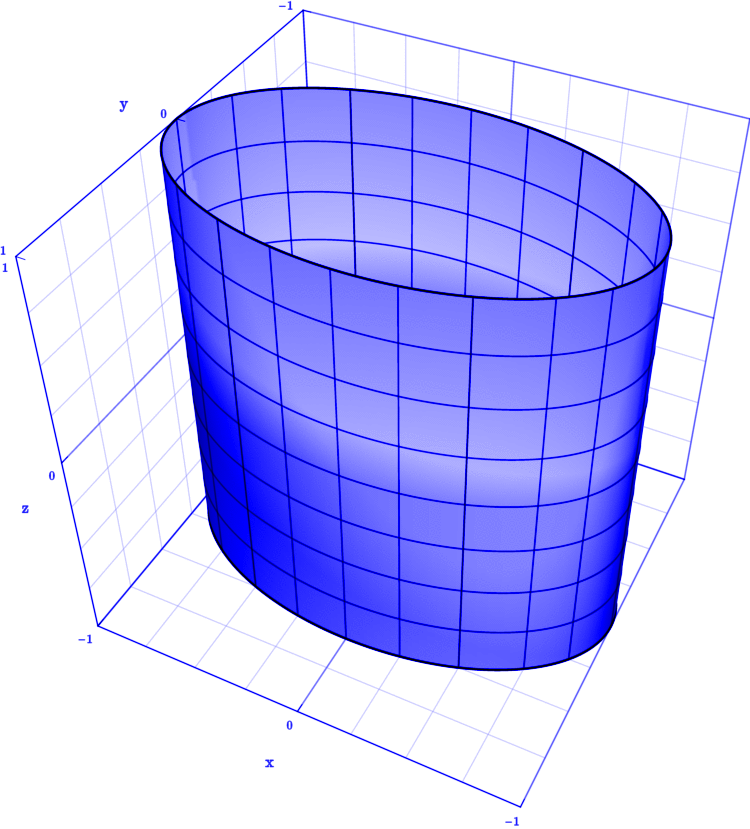
\includegraphics[height=0.090\columnwidth]{img/q7.png}}
\fbox{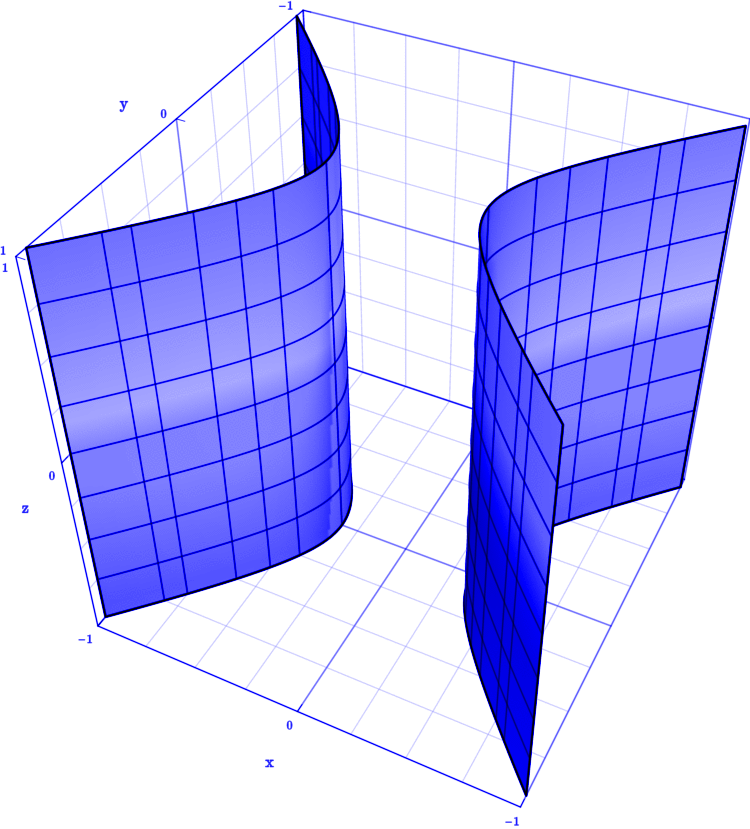
\includegraphics[height=0.090\columnwidth]{img/q8.png}}
\fbox{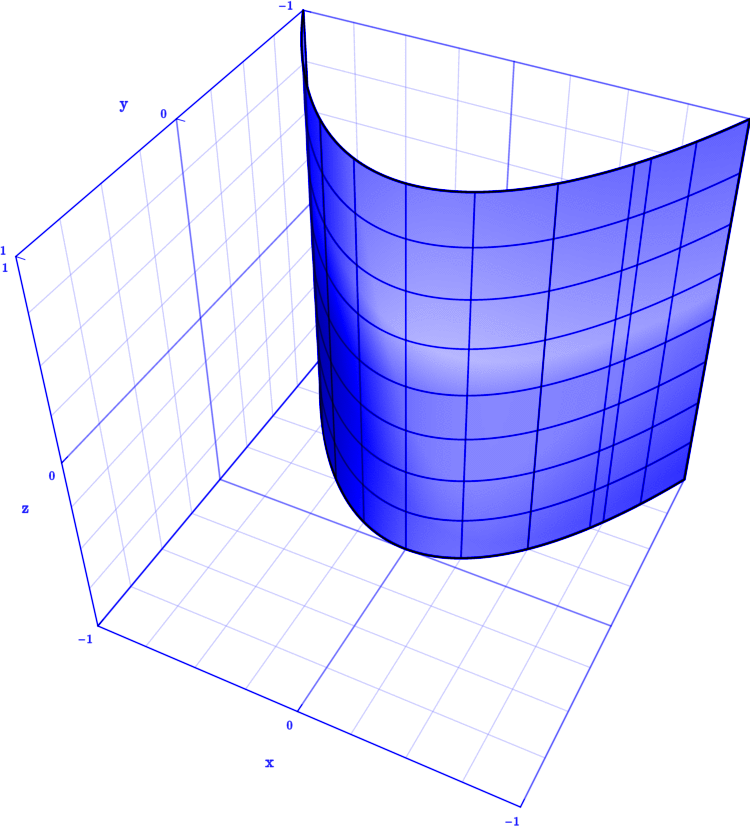
\includegraphics[height=0.090\columnwidth]{img/q9.png}}
\fbox{
\includegraphics[height=0.090\columnwidth]{img/q0.png}}
\end{center}

\begin{multicols}{2}
\begin{enumx} 
\item $x^2 + y^2 + z^2 = 1$ \hfill elipsoida
\item $x^2 + y^2 - z^2 = 1$ \hfill hiperboloida 1-powłokowa
\item $x^2 - y^2 - z^2 = 1$ \hfill hiperboloida 2-powłokowa
\item $x^2 + y^2 - z = 0$ \hfill paraboloida eliptyczna
\item $x^2 - y^2 - z = 0$ \hfill paraboloida hiperboliczna
\item $x^2 + y^2 - z^2 = 0$ \hfill stożek eliptyczny
\item $x^2 + y^2 = 1$ \hfill walec eliptyczny
\item $x^2 - y^2 = 1$ \hfill walec hiperboliczny
\item $x^2 - y = 0$ \hfill walec paraboliczny
\item inne są wypaczone bardzo (punkt, prosta, płaszczyzny). % x^2 + y^2 + z^2 = 0, x^2 + y^2 = 0, x^2 - y^2 = 0, x^2 = 1, x^2 = 0
\end{enumx}
\end{multicols}
   
Jeśli \prawo{253} $V$, p. liniowa nad $\mathfrak K$, ma wymiar $n+1$, to \wcht{p. rzutową} $\mathbb P(V)$ jest zbiór wszystkich prostych wektorowych (podprzestrzeni wymiaru $1$).
Jeśli $V$ ma bazę $(e_0, \dots, e_n)$ i $x = \sum_{k=0}^n \xi_k e_k \in V \setminus \{0\}$, to $\xi_k$ są \wcht{współrzędnymi jednorodnymi} dla $x$.
W $V$ mamy podprzestrzeń $V_0$, $\langle e_1, \dots, e_n\rangle$, a w afinicznej $(\mathbb A = V, V)$ hiperpłaszczyznę: $\mathbb A_0 = e_0 + V_0$.
Afiniczna $\mathbb A_0$ z odwzorowaniem $\Phi_0$ ($\langle x \rangle \mapsto \langle x \rangle \cap \mathbb A_0$ obcięte do $\mathbb P(V) \setminus \mathbb P(V_0)$) to \wcht{mapa afiniczna}; zbiór $\mathbb P(V_0)$ składa się z ,,punktów w nieskończoności''.
\emph{Przekształcenia rzutowe tworzą pełną grupę}.
\emph{Geometria rzutowa}.
\emph{Dwustosunek}.

\wcht{Stożek izotropowy} $C$: \prawo{2 / 54} jądro $q$, formy kwadratowej na p. liniowej $V$ wymiaru $n + 1 \ge 2$ nad $\R$.
Jeżeli jądro to jest nietrywialne (różne od $\{0\}$), to obraz $C \setminus \{0\}$ przez kanoniczne $\pi \colon V \setminus \{0\} \to \mathbb P(V)$ jest \wcht{kwadryką rzutową}.
\wcht{Podprzestrzeń podwójna}: ten sam obraz, o ile jest on podprzestrzenią rzutową wymiaru $n - r$ (dla $r < n$).
Każda niepodwójna kwadryka w p. rzutowej $\mathbb P(V)$ wymiaru $n$ jest równoważna rzutowo dokładnie jednej o równaniu $x_0^2 + \dots + x_s^2 - x_{s+1}^2 - \dots  - x_r^2 = 0$, gdzie $[r/2] \le s < r$.